\chapter{Background}
This chapter presents a brief overview of relevant literature on speech intelligibility, prosody, and talker familiarity.  Because the experiments described in this thesis involve speech obscured by background noise, a review of auditory masking research is also given.  The discussion of talker familiarity touches on both short-term familiarity (\ie training and exposure studies) and long-term familiarity.  Finally, the discussion of prosody focuses on pitch, loudness, and duration as they relate to speech perception.

\section{Auditory masking}
It is well known that auditory masking is dependent on both the spectrotemporal characteristics of the masking sound as well as its relationship to the target sound.  %\citet{Miller1947} puts it succinctly: “...the masking of speech [depends] on three characteristics of the masking sound: (1) its intensity relative to the intensity of the speech, (2) its acoustic spectrum, and (3) its temporal continuity” \citep[106]{Miller1947}.  
Even the early experiments of \citet{WegelLane1924} — which involve only pure-tone targets and maskers — reveal the importance of the relationship between target and masker sounds.  Those experiments demonstrate that, regardless of the target tone frequency, masker tones \emph{close in frequency to the target tone} are the best maskers (except when the frequencies are so similar as to cause beating).  

In the nearly 90 years since, numerous aspects of the target-masker relationship have been investigated and found to impact the masking of speech.  In this section, those factors are discussed in terms of the division between energetic and informational masking, with informational masking split into two broad categories: masking due to target-masker similarity within a stimulus, and masking due to unpredictability (and, consequently, listener uncertainty) across stimuli (following \citealt{KiddEtAl2002} \etseq).  It is acknowledged that the terms \term{energetic masking} and \term{informational masking} have historically been somewhat ill-defined \citep[cf. discussions in][]{DurlachEtAl2003a, Watson2005}, though for present purposes they will suffice as an organizing principle for review of the literature.% (since more recent terms like \term{peripheral masking} or \term{central masking} \citep{DurlachEtAl2003a} are not always obviously appropriate to describe older studies).

\subsection{Energetic and informational masking\label{sec:InfoMasking}}
Early masking experiments with speech targets were often performed with noise maskers \citep[\eg][]{HawkinsStevens1950,Tolhurst1957b,PollackPickett1958}.  The noise used was typically a random (gaussian) signal, usually without any amplitude modulation (\term{stationary maskers}) or frequency shaping (\term{white noise maskers}).  Masking due to any such random signal is typically termed \term{energetic masking}, reflecting the idea that the masking is a consequence of elevated signal detection thresholds in the auditory filters of the cochlea (cf. the discussion in \citealt[96–97]{Moore2008}, and the notion of \term{peripheral masking} proposed by \citealt{DurlachEtAl2003a}).  However, most everyday situations involve listening to speech in the presence of competing speech streams — a situation poorly modeled by stationary white noise maskers, since real speech is both amplitude modulated and frequency shaped (indeed, the frequency shaping of speech is itself dynamic).

\label{par:Glimpsing}When speech is used as a masker, the amplitude modulations in the masker speech create temporal variations in \ac{snr} of the signal that can offer \term{glimpses} of the target stream \citep{FestenPlomp1990}.  The existence of such glimpses make speech a (potentially) worse masker than stationary noise, since listeners can use the glimpses to reconstruct neighboring spans of the target stream that are less clearly heard.\footnotemark{}  Glimpses can also occur with amplitude-modulated random noise maskers, and if noise maskers are both amplitude-modulated and frequency-shaped so as to be maximally comparable to speech maskers, what we find is that target perception accuracy is lower when masked by speech than by noise \citep[\eg][]{CarhartEtAl1969,LewisEtAl1988,SimpsonCooke2005}.  The additional masking present in speech maskers is termed \term{informational masking} (less commonly: \term{perceptual masking}), and is usually attributed to the (linguistic) information contained in the masker signal competing for language processing resources at higher levels of the auditory and language processing streams in the brain \citep{DurlachEtAl2003a,xxx}.
\footnotetext{The reconstruction of surrounding context may be based on lexical knowledge, phonotactics, transitional probabilities between words, contextual probabilities based on semantics, etc. \citep{xxx}.}

As \citet{Cooke2006} points out, glimpsing is not necessarily a strictly temporal phenomenon: there can be spectral regions of the target signal that are relatively more or less obscured by the masker signal at a given point in time.  For example, the formants of a relatively loud vowel might in fact exceed the intensity of the masker noise, especially at relatively low \ac{snr}s (see Figure~\ref{fig:PartialGlimpsing}).

\begin{figure}[htbp]
	\begin{centering}
	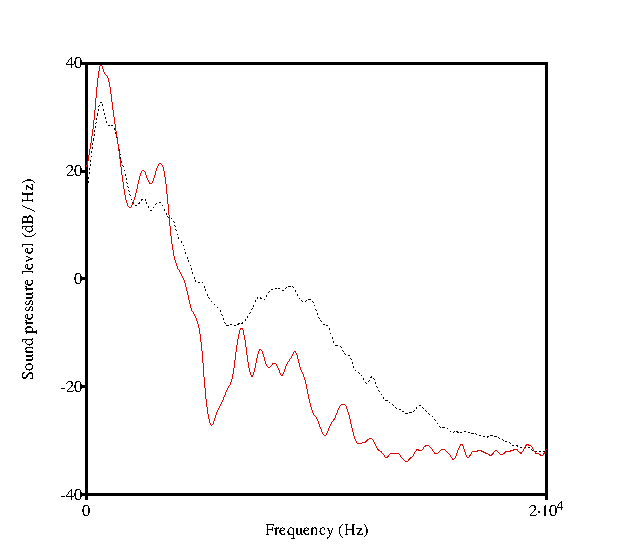
\includegraphics{figures/partialGlimpsing.eps}
	\caption[Partial glimpsing of an {[ɑ]} vowel]{Partial glimpsing, illustrated by power spectrum of an [ɑ] vowel (solid red line) poking above the long-term average spectrum of the sentence from which the [ɑ] was extracted (dotted black line), at a signal to noise ratio of 0 dB. Both spectra have undergone cepstral smoothing with a 500 Hz bandwidth.\label{fig:PartialGlimpsing}}
	\end{centering}
\end{figure}

One can simultaneously reduce glimpses and decrease the recognizability of background speech by increasing the total number of background speech streams (\ie by using a \term{multitalker babble masker}).  Most work using babble maskers shows that the degree of masking increases as the number of competing speech signals increases \citep[\eg][]{Miller1947, BrungartEtAl2001}.  However, recent research suggests that indefinitely increasing the number of talkers does not necessarily increase masking: total masking seems to plateau around 6–8 background talkers; further increasing the number of talkers causes the masking to recede back to the lower level seen with stationary, frequency-shaped random noise \citep{SimpsonCooke2005}.  This finding can be understood as the result of an interaction between energetic and informational masking: as the number of background talkers increases, the spectrotemporal glimpses tend to decrease (increasing energetic masking), while the informational content of any individual masker voice becomes increasingly obscured by competing background talkers (decreasing informational masking).  Put another way, as the number of talkers continues to increase, spectrotemporal variation decreases and the babble masker more and more closely approximates the long-term average spectrum of speech \citep{SimpsonCooke2005}.

\subsection{Target-masker similarity\label{sec:similarity}}
Another important factor in the perception of speech in noise is the similarity of the masker and target signals.  “Similarity” may refer to fine-grained comparisons of spectral similarity (\eg tone complexes masked by similar tone complexes, as in \citealt{LeeRichards2011}), or to more abstract properties of the signals.\footnotemark{}  As one example of a more abstract signal property, the perceived spatial origin of the competing speech streams can be construed as a form of target-masker (dis)similarity, and numerous studies have shown a release from masking due to spatial separation between the target and masker streams \citep[\eg][]{FreymanEtAl1999, BrungartSimpson2002, FreymanEtAl2004, GallunEtAl2005, KiddEtAl2005a, JohnstoneLitovsky2006}.  Likewise, \citet{Brungart2001} showed that similarity between the voices in the target and masker speech streams was also predictive of masking: perception of the target stream is most difficult when the voices in the target and masker streams belong to the same person, moderately difficult when the voices belong to same-gendered talkers, and least difficult when the target and masker voices belong to a gender-mismatched pair (a finding later replicated by \citealt{HelferFreyman2008}).
\footnotetext{Cf. the distinction in \citet{Watson2005} between target-masker \term{structural similarity} and target-masker \term{representational similarity}.}

Similarity in the language of the target and masker streams also affects masking.  For example, native English listeners perform better on English target speech when the masker speech is Spanish \citep{GarciaLecumberriCooke2006}, Dutch \citep{BrouwerEtAl2012}, or Modern Standard Chinese \citep{VanEngenBradlow2007} rather than English.  Analagous experiments by \citet{RhebergenEtAl2005} showed similar effects for Dutch listeners exposed to Dutch target speech with either Dutch or Swedish maskers.  

Informational masking also seems to be affected by the accessibility or perceptibility of the information in the masker stream(s).  For example, the release from masking seen with mismatched target and masker languages is smaller in cases where the masker language is comprehensible to the listener \citep{VanEngen2010}.  Related findings by \citet{CalandruccioEtAl2010} also support the relevance of masker accessibility or perceptibility: their study showed that for English target speech and native English-speaking listeners, native English masks better than foreign-accented English.\footnotemark{}  Perhaps most interestingly, \citet{BrouwerEtAl2012} showed that semantically anomalous English sentences provide less masking than semantically coherent ones, but no similar effect was found for English targets masked by semantically well-formed and anomalous Dutch speech.  Perhaps most convincingly, informational masking (indexed by reaction time) has been shown to correlate with the lexical frequency of the words in the masker speech \citep{BoulengerEtAl2010}.
\footnotetext{Corollary experiments confirmed that the difference was due to variation in the intelligibility of the background talker, not spectrotemporal differences between the masker streams \citep{CalandruccioEtAl2010}.}

Taken together, these findings seem to support the view that some cases of informational masking can be explained by \term{lexical pop-out} of specific words in the masker speech.  According to such an explanation, comprehensible background speech can compete with target perception relatively late in the auditory processing stream (\ie at the point at which lexemes are recognized or accessed).  In contrast (so the explanation goes), incomprehensible background speech (such as foreign-language babble) is unlikely to trigger lexical competition, except by dint of accidental similarity to native words (a very low probability occurrence).  Experiments comparing normal to time-reversed masker speech also provide support for the lexical pop-out explanation of informational masking (\eg \citealt{HoenEtAl2007}, though cf. \citealt{RhebergenEtAl2005} for a review of issues related to forward masking in time-reversed speech).

This reasoning can be extended to the findings of \citeauthor{CalandruccioEtAl2010} showing that high-intelligibility (native) speech masks better than low-intelligibility (foreign-accented) speech, on the assumption that words are high-intelligibility precisely because they more readily trigger lexical activation (due to, \eg greater cue redunancy).  The findings of \citeauthor{BrouwerEtAl2012} (showing weaker masking from babble comprising semantically anomalous sentences) might also be explained by appeal to lexical pop-out, though the explanation is somewhat more tenuous: a lack of semantic priming in the masker sentences would decrease the likelihood of lexical activations due to words in the masker stream, thereby reducing lexical competition from the background stream.  Regardless, many of the findings mentioned above can also be explained by appeal to stimulus uncertainty, discussed in the following section. %Moreover, the phenomenon of lexical popout presumably becomes less likely as the number of competing speech streams increases, so if differences between maskers of differing language, intelligibility, or semantic content are found with high numbers of background talkers, some other explanation must be proposed.

\subsection{Masking and listener uncertainty\label{sec:uncertainty}}
Another apparent source of informational masking is the trial-to-trial regularity of the target and masker stimuli.  Experiments with pure-tone targets and pure-tone complexes as maskers have shown significant release from masking when masker is held constant for the two intervals of each trial, even when the masker still varies spectrotemporally between trials \citep{NeffGreen1987, NeffCallahan1988}.  Similar results (again using tone complexes) have been obtained for masker spatial location \citep{FanEtAl2008} and temporal location \citep{BoninoLeibold2008}.  Such results suggest that some notion of listener uncertainty (or conversely, stimulus predictability) is important to a full account of informational masking.  Additionally, stimulus uncertainty has been shown to interact with target-masker similarity, such that masking under conditions of stimulus uncertainty is stronger when target and masker are more similar \citep{DurlachEtAl2003b}.

Early studies of listener uncertainty using speech stimuli showed higher word-recognition scores for blockwise presentation of a single talker compared to mixed-talker blocks \citep{SommersEtAl1994}, suggesting that listeners can accomodate (or \term{tune in}) to a particular voice when talker identity is predictable (a finding replicated in \citealt{BrungartSimpson2004} and \citealt{EricsonEtAl2004}; cf. also the discussion of training studies in Section~\ref{sec:Training}).  
%In contrast, trial-to-trial variability in overall amplitude of stimuli does not seem to affect speech perception \citep{SommersEtAl1994}.  
Similar results are seen when holding fixed other dimensions of the stimuli.  For example, in a closed-set response task using the \ac{crm} corpus, holding fixed the semantic content of the masker stream leads to a release from masking even when the voice speaking the masker phrase changes trial-to-trial \citep{BrungartSimpson2004}.  Other studies have shown that uncertainty about the spatial location of the target speech (in the presence of competing, spatially distinct speech streams) results in dramatically lower target perception success than cases where the location of the target speech is known \citep{EricsonEtAl2004, KiddEtAl2005a}.  However, the generalizability of findings based on small-vocabulary response sets is uncertain: a study using nonsense sentences as targets and maskers found little to no effect of stimulus variation (and hence listener uncertainty) in \ac{snr}, talker identity in the masking stream, or masker content \citep{FreymanEtAl2007}.

In general, experiments exploring stimulus uncertainty using speech maskers have been less common than studies using nonspeech stimuli, presumably due to the difficulty of controlling and quantifying the spectrotemporal similarity of speech maskers (as can be done fairly readily with tone complexes).  Despite this relative lack of research, stimulus uncertainty may turn out to play a role in explaining previous findings thought to be related to target-masker similarity.  For example, increased masking from native- vs foreign-language babble maskers \citep[\eg][]{RhebergenEtAl2005, GarciaLecumberriCooke2006, VanEngenBradlow2007, BrouwerEtAl2012} might be explained as a difference in stimulus uncertainty: in the foreign-language babble, the accessible semantic content is constant and predictable (\ie null) whereas the native-language babble has varying semantic content (in that the identity and timing of words that pop out of the babble varies from trial to trial).  Further research is needed to disentangle the roles of similarity and uncertainty under such circumstances.  %Similarly, the weaker masking due to semantically anomalous native-language babble \citep{BrouwerEtAl2012} could be construed as a stimulus uncertainty problem, 

% TODO: conclusion/transition?

\section{Intelligibility}
This section first reviews past findings on intelligibility related to four commonly measured acoustic dimensions of speech: vowel formant frequencies, duration, intensity, and pitch.  This is followed by a discussion of segmental features and cues, particularly as related to the phenomena of clear speech, speech reduction, and Lombard effects.  Next, these dimensions of speech are related to talker characteristics such as gender, dialect, sociolect, and foreign accent.  The section concludes with a brief discussion of the role of the listener in intelligibility, focusing on peripheral hearing loss and age-related cognitive decline.%, with brief mention of specific language impairment (SLI) and central auditory processing disorder (CAPD).

%\subsection{Acoustic dimensions of speech}
%A variety of studies have examined the acoustic dimensions of speech that might be predictive of intelligibility in noise.  Unfortunately, it is hard to find a consensus in the literature: the acoustic dimensions tested and the significance reported are not consistent across studies.  Here I review the major findings relating to vowel formant frequencies, duration, intensity, and pitch.

\subsection{Intelligibility and vowel formant frequencies\label{sec:IntelVowel}}
Much research supports the idea that intelligibility is linked to properties of the F2×F1 vowel space \citep[\eg][]{BondMoore1994, BradlowEtAl1996, HazanMarkham2004, Neel2008, McCloyEtAl2013}, though precisely which properties of the vowel space correlate with intelligibility is still an unresolved question.  There seems to be consistent evidence for the overall size of the vowel space as a predictor of intelligibility, though different studies have used different metrics of vowel space size.  Size-related measures reported to positively correlate with intelligibility include F1 range \citep{BradlowEtAl1996}, F2 range \citep{HazanMarkham2004}, mean distance of vowel tokens from the center of the vowel space \citep{BradlowEtAl1996, McCloyEtAl2013}, area of polygon formed by vowel means (\citealt{BradlowEtAl1996}: /i~o~a/; \citealt{Neel2008}: /i~æ~ɑ~u/;  \citealt{McCloyEtAl2012}: /i~ɪ~e~ɛ~æ~a~ɔ~o~ʊ~u/), and area of the convex hull encompassing all vowel tokens \citep{McCloyEtAl2013}.  

The area of the convex hull is arguably the most appropriate metric of vowel space expansion, since measures like F1 and F2 range may be more sensitive to dialectal variation, and values for mean distance from center will vary dramatically depending on which vowels are included in the analysis (see \citealt{McCloyEtAl2013} for discussion).  More research is needed to determine which of these metrics is most stable across languages and talker groups, and which most reliably indexes differences in intelligibility.

Another important aspect of the F2×F1 vowel space is the degree of vowel phoneme overlap or \term{phonemic crowding}.  Phonemic crowding can be indexed by the total repulsive force of the vowel system \citep[see][]{McCloyEtAl2013}.  Mean vowel cluster size indexes the within-category variability of the vowel phonemes, which is related to (and likely to covary with) phonemic crowding \citep{McCloyEtAl2013}.  
% “Mean vowel cluster size was calculated for each talker as the mean of the areas of the 95\% confidence ellipses for each vowel category (based on bivariate normal density contours).  Low values of cluster size are associated with low degrees of within-category variation and therefore (we predict) a more predictable perceptual target and higher intelligibility.”

% TODO: say something about normalization?

%From these 15 sentences the average pitch range magnitude was calculated for each talker,\footnote{The choice to use mean size of pitch range rather than absolute pitch range was motivated by the fact that a given sentence may be uttered in a fairly monotone fashion even by a talker that has a large overall pitch range.  Thus we reason that a talker's \textit{typical} range across utterances is more indicative of their linguistic use of pitch than their \textit{potential} or \textit{maximal} range.  Ideally, pitch range would be a stimulus-level predictor rather than a talker-level aggregate, but reliable measures of pitch range for all 3600 stimuli was not possible given the need for hand correction (stemming from the difficulty of automatic pulse detection and pitch tracking algorithms in dealing with creaky voicing).} as well as the mean absolute value of rate of change in pitch (“pitch dynamicity,” cf. measures of “pitch velocity” used in \citealt{GauthierEtAl2007b, GauthierEtAl2007a, GauthierEtAl2009}).  This yielded a total of 300 pitch tracks for data analysis (15 per talker × 20 talkers).

\subsection[Intelligibility and duration]{Intelligibility and duration: Speech rate and speech rhythm\label{sec:IntelDur}}
One of the earliest studies of the relation between intelligibility and speech rate was performed by \citet{Tolhurst1957a}, who found a significant effect for duration among three speech styles (prolonged, normal, and staccato) in an analysis of variance test.  In more recent studies, evidence has been mixed as to whether speech rate is predictive of intelligibility.  For example, \citet{SommersEtAl1994} found a significant effect of variation in speech rate on intelligibility, suggesting that speech rate is one of the factors relevant to masking due to listener uncertainty.  In contrast, \citet{BradlowEtAl1996} found no correlation between mean sentence duration and intelligibility, and \citet{KrauseBraida2002} found that the intelligibility difference between clear and conversational speech is apparently independent of speaking rate.  Examining word durations, \citet{BondMoore1994} found differences in isolated word durations between two talkers of varying intelligibility, but not in words in sentential context.  Finally, in modern a study echoing \citet{Tolhurst1957a}, \citet{MayoEtAl2012} examined plain, infant-directed, computer-directed, foreigner-directed, and shouted speech, finding a correlation between sentence duration and word error rate across speech styles, as well as significant segment length differences across speech styles for stops, fricatives, nasals, vowels, and diphthongs (but not affricates, liquids or glides).  Their findings suggest that “much of the prosody-related intelligibility gain comes from durational increases” \citep{MayoEtAl2012}.

To the extent that duration covaries with other dimensions of linguistic variability (\eg segmental reduction), it is unsurprising that duration can be predictive of speech intelligibility.  However, it remains unclear whether measurements of duration reflect a genuine percept in the speech perception process, or are merely a convenient surrogate for other, harder-to-measure factors like segmental reduction or the occurence of spectrotemporal glimpsing.

There is also some evidence that patterns of duration (\ie rhythm) can contribute to speech intelligibility.  The proper description and classification of linguistic rhythm has been a long-standing debate in the field, and a thorough rehashing of those issues is beyond our purposes here.\footnotemark{}  Nonetheless, two studies bear reporting here for their relation to intelligibility.  First, with regard to duration in foreign-accented speech, \citet{QueneVanDelft2010} found that the speech reception thresholds (\ac{srt}) of high-intelligibility non-native Dutch sentences were improved when the sentences were resynthesized to match the durational patterns of a native Dutch speaker, while the \ac{srt} of native Dutch speech was degraded when the native sentence was resynthesized to have the durational patterns of non-native speech.  Second, in a 2×2 design investigating native duration patterns and syllable-isochronous duration patterns where all stimuli had been monotonized, it was found that target speech perception was above chance only when the target had native-like duration patterns and the competing speech had syllable-isochronous duration patterns \citep{CushingDellwo2010}.  In other words, subjects performed near chance when either the masker had native-like durations, or the target had syllable-isochronous durations.  
\footnotetext{A succinct summary of the issues and evidence regarding the classification of linguistic rhythm can be found in \citep{Ramus2002}.}

Both of those studies suggest an intelligibility benefit for sentence-length stimuli with native-like durational patterns.  The relationship between rhythmic variations (\eg between native-like and non-native-like rhythms) and summary measures of duration (\eg mean sentence length) is not well understood (cf. \citealt{Ramus2002}).  One recent study looking at differences in temporal structure between conversational and clear speech primarily found differences in occurrences of vowel and consonant reduction and deletion, leading to differences in the number of prosodic phrases, but an overall consistency across speech styles in the ratio of consonantal to vocalic stretches and the variability of each \citep{SmiljanicBradlow2008}.  In other words, consonants and vowels were both subject to durational reduction in conversational style (in roughly equal measure), and the variability in consonant and vowel duration remained constant across speaking styles (relative to the overall speech rate).

Of course, there is more to rhythm than simply duration patterns, and neither \citet{QueneVanDelft2010} nor \citet{CushingDellwo2010} accounted for differences in intensity patterns between the native and non-native conditions (though both did equate the mean intensities of all stimuli).  A discussion of the relation between intensity and intelligibility follows in Section~\ref{sec:IntelIntens}; unfortunately there will be little to say about rhythmic patterns of intensity as related to speech intelligibility, as such research is still in its infancy (though see \citealt{TilsenJohnson2008} for a recent inroad into quantifying speech rhythm through Fourier analysis).

% see also:
% \citep{Fry1955}: duration as cue to English word stress (measured productions and synthesized perception experiment)
% \citep{Klatt1976, WightmanEtAl1992}: linguistic use of duration in general
% \citep{RamusEtAl1999}: acoustic correlates of rhythm
% \citep{RaoSmiljanic2011}: age, clear speech & rhythm in English and Croatian
% \citep{LiuZeng2006}: time-compression and silence addition to change speech rate of clear and conversational speech.
% \citep{SundaraScutellaro2011}: rhythmic distance affects bilingual infants’ acquisition.
% \citep{DellwoHagmann2011}: the processes that underly the perception of duration seem to be sensitive to linguistic structure; contrastive length affects duration percepts.

\subsection[Intelligibility and intensity]{Intelligibility and intensity: Audibility and \ac{snr}\label{sec:IntelIntens}}
When considering the relationship between the intensity of speech and its intelligibility, the most obvious consideration is whether the speech is loud enough to be above the listener’s auditory thresholds in the relevant frequency regions.  In other words, for speech to be intelligible it must be audible.  In real-world settings this is affected not only by the source power of the talker’s speech, but also by the distance between talker and listener, their relative head orientations, the presence of background noise, and any irregularities in auditory thresholds of the listener (\ie hearing loss or congenital deficit).

In contrast, laboratory settings offer controlled signal levels, minimal background noise, and minimal or no effect of head orientation due to the use of headphones (or the use of gaze fixation points with free-field sound sources).  Irregularities in auditory thresholds can also be accounted for by audiometric testing of listeners.  Thus in the laboratory audibility is well within the experimenter’s control, and the most important audibility consideration becomes the intensity contour of the target signal itself, especially in relation to different masking signals.% and \ac{rms} normalization.

In all speech stimuli there is considerable variation in intensity across the span of the stimulus.  Some of this variation is due to inherent differences in intensity of different speech sounds (\eg vowels tend to be louder than nasals; [f] is nearly always quieter than [s]; \citealt{sowl}).  In sentence-length or longer stimuli, there is also variation in the mean intensity of each word.  This variation is not random, but rather is determined by linguistic properties of the speech, in particular lexical stress and phrasal accent \citep{Fry1955, SluijterVanHeuven1996, PlagEtAl2011}.  There is also a \comment{cross-linguistic?} tendency for words at the ends of utterances to be quieter than words near the start of the utterance \citep{Ladefoged1967, StrikBoves1995, TrouvainEtAl1998}.  This can lead to differences in \ac{snr} across the span of the utterance, and increase or decrease the probability of glimpsing a particular word depending on its position in the sentence (cf. Section~\ref{par:Glimpsing}).  

% see also:
% \citep{Fry1955}: intensity as cue to English word stress (measured productions and synthesized perception experiment)
% \citep{BondMoore1994}: no differences in intensity for the three differently intelligible talkers.  
% \citep{TilsenJohnson2008}: Methods for measuring rhythm. 

\subsection[Intelligibility and pitch]{Intelligibility and pitch: Gender and voice quality}
A number of studies have looked for a significant relationship between the fundamental frequency (\fo) of speech and speech intelligibility.  Typically, what is found is that static measures of pitch such as mean \fo do not correlate with speech intelligibility, whereas measures that reflect a talker’s dynamic use of pitch are more relevant.  For example, both \citet{BradlowEtAl1996} and \citet{McCloyEtAl2013} report a positive correlation between \fo range and intelligibility, and \citet{McCloyEtAl2013} also report a significant effect for rate of change of \fo (\term{pitch dynamicity}, cf. \citealt{GauthierEtAl2007b, GauthierEtAl2007a, GauthierEtAl2009}).  \citet{BinnsCulling2007} report a significant increase in speech reception threshold in an English competing speech task when the \fo contour of target speech is flattened or inverted, but no effect when the masker speech is similarly manipulated; \citet{WatsonSchlauch2008} report similar results for speech with flattened \fo in white noise.  Unsurprisingly, flattening pitch contours also impacts intelligibility in lexical tone languages like Modern Standard Chinese \citep{PatelEtAl2010}.

However, both of the measures just discussed — \fo range and pitch dynamicity — are intuitively associated with more a animated speech style, which typically also involves changes in other dimensions that are relevant to intelligibility (\viz intensity, duration, and vowel formant frequencies).  They are also highly correlated with talker gender, and any of those dimensions may be exploited for sociolinguistic marking of gender \citep{xxx}, in ways that are not necessarily consistent in different languages or dialects \citep{xxx}.  Pitch accent, boundary tone, and pause distribution also varies regionally and with gender \citep{ClopperSmiljanic2011}.  These correlations among intelligibility and the acoustic dimensions of speech are thus difficult to disentangle, and any individual finding should be interpreted cautiously.

A final issue related to fundamental frequency concerns voice quality or phonation.  In cases where pitch drops at the end of an utterance, irregular phonation (\term{creaky voicing}) often occurs \citep[\eg][]{Kreiman1982}.  \comment{this paragraph unfinished...}

\subsection{Segmental cues}
Intelligibility in various simulated environments w/r/t vowel ID, consonant contrasts in voicing, continuance, place \citep{CoxEtAl1987}.  
presence of stop release bursts \citep{PichenyEtAl1986, LiLoizou2008}

\subsubsection{redundancy}
Smooth signal hypothesis, etc.

\subsubsection{Clear speech and reduced speech}
\comment{This part is still rather sketchy.}
Definition of clear speech.  
Early work establishing an intelligibility difference between clear and conversational speech and showing errors in perceiving conversational speech in both consonant and vowel perception \citep{PichenyEtAl1985}.  So why is clear speech more intelligible?  Clear speech has less vowel reduction and more word-final stop releases \citep{PichenyEtAl1986}.  Taken together with findings that vowel reduction and release bursts are predictive of intelligibility across talkers \citep{xxx,LiLoizou2008}, it is likely that the intelligibility difference between clear and conversational speech can be at least partially explained by differences on those dimensions.  Clear speech is also slower than conversational speech, due to both more pauses and longer word durations \citep{PichenyEtAl1986}.  However, early attempts to determine the contribution of speech rate to the intelligibility of clear speech have met with mixed results, due at least in part to the processing artifacts that arise when manipulating stimulus duration \citep{PichenyEtAl1989, UchanskiEtAl1996, LiuZeng2006}.  See Section~\ref{sec:StimDesign} for further discussion.

Time-compression / silence addition to change speech rate of clear and conversational speech \citep{LiuZeng2006}.  
Clear speech benefits native and non-native talkers and listeners \citep{SmiljanicBradlow2011}.  
Temporal structure of clear / conversational speech \citep{SmiljanicBradlow2008}.  
Clear speech acoustics \citep{KrauseBraida2004}.  
Clear speech envelope \citep{KrauseBraida2009}.  
“Read, clear speech showed more extreme changes in median F0, F0 range, and speaking rate than speech produced to counter the effects of a challenging listening condition” \citep{HazanBaker2011}.

\subsubsection{Lombard speech}
Amplitude, duration, pitch and formant frequencies change in lombard task \citep{SummersEtAl1988}.

\subsection{Talker characteristics}

\subsubsection{Gender}
talker gender and pitch range \citep[\eg][]{BradlowEtAl1996}

\subsubsection{Dialect, sociolect, \& foreign accent}
Setting aside real-world situations (accommodation,etc)...  Lombard, unintentionally clear speech, intentionally clear speech, register.  foreign accent \citep{SmiljanicBradlow2011}

\subsection{Listener characteristics}
In general human auditory system looks like xxx, with little variability.  However, hearing loss, cognitive decline, etc.  Other things to possibly include?  Many have already been discussed under "masking".  Maybe just a paragraph to say "talker/listener relationship etc etc, already discussed under masking, not really intelligibility per se, since it has to do with listener as well as talker."  Re: cognitive decline, discuss \citep{MattysEtAl2009}, which showed that energetic masking increased reliance on acoustic cues, whereas cognitive load (info masking) increased reliance on lexico-semantic cues. 

%\begin{itm}
%	\item{target talker/listener dialect mismatch}
%	\item{target talker nonnative accent}
%	\item{native vs non-native listeners \citep{CookeEtAl2008, CookeEtAl2010, BrouwerEtAl2012}}
%	\item{It has been shown that foreign babble masks less well than native babble \citep{RhebergenEtAl2005,VanEngenBradlow2007,WuEtAl2011}.  At least in some cases, native-language babble masking is due to due to distracting lexical pop-out \citep{HoenEtAl2007}.  However, it is unclear whether differences are solely attributable to lexical interference from the native background speech, or whether other aspects of the native and foreign speech might be contributing to differential masking ability (\eg familiar vs unfamiliar phones, rhythms, or intonation contours). Rhebergen et al's study is particularly problematic, since their native-language masker (Dutch) was time-scaled using PSOLA to match the speech rate of the (unmodified) foreign-language masker (Swedish).}
%\end{itm}

\subsection{Signal content characteristics}
\begin{itm}
	\item{lexical effects \citep{HoenEtAl2007, BoulengerEtAl2010, BrouwerEtAl2012}}
	\item{lexical frequency: When the masker is a speech stream, high-frequency words are more likely than low-frequency words to pop out of the background and cause distraction (\ie slow reaction time, or mishear target word for background competitor) \citep{BoulengerEtAl2010}.}
	\item{neighborhood density}
	\item{contextual probability / predictability.  For example, \citet{LewisEtAl1988} showed that words that are predictable from context are harder to mask, in that they are recoverable (or at least guessable) at lower \ac{snr}s than the same words in low-context sentences.  At the same time, words that are predictable from context are typically articulated less distinctively, as though the talker were balancing their own articulatory effort with expectations that the listener is paying attention and can recover some words more easily than others \citep{Wright2004}.  }
	\item{Lexical activation (\textsc{aka}, word recognition) also helps when learning to recognize talkers: if the talkers are speaking an unfamiliar language, it is harder to learn to distinguish their voices \citep{PerrachioneWong2007}.}
\end{itm}


%A synthesis of this research leads to the conclusion that virtually every aspect of a target or masker stimulus is potentially relevant to speech perception, including many facets of speech that are often difficult to balance or control for (\eg talker voice quality, timing of glimpses in the masker envelope, lexical frequency and semantic predictability of target words, familiarity with the talker’s voice or dialect, etc).


\section{Familiarity}
some introductory text about familiarity.  NygaardEtAl1994, NygaardEtAl1999, Yonan\&Sommers2000

\subsection{Training studies\label{sec:Training}}
\citep{VanEngen2012}.  
Training talker ID on English vs German words, testing on English words, only English training worked \citep{LeviEtAl2011}.  Proposed explanation is “linguistically relevant contrasts”.

\subsection{Long-term familiarity studies}
college prof study \citep{NewmanEvers2007}.  Long-term partners/friends \citep{SouzaEtAl2013}.

\subsection{Priming studies}
priming first few words of target utterance \citep{FreymanEtAl2004}.  priming target words in a simultaneous unattended contralateral speech stream \citep{RivenezEtAl2006}.  priming target talker voice and spatial location (=familiarity) \citep{KiddEtAl2005a, KitterickEtAl2010}.  "Implicit auditory priming" \citep{Sommers1999}.

